\documentclass[9pt, mathserif]{beamer}
\usefonttheme{serif}
\usetheme{Berlin}
\usecolortheme{seagull}
\usepackage[utf8]{inputenc}
\usepackage{amsfonts}
\usepackage{lmodern}
\usepackage{amsmath}
\usepackage{geometry}
\usepackage{graphicx}
\usepackage{tikz}
\usepackage{url}
\usepackage{geometry}
\usepackage{bm}
\usepackage{physics}
\usepackage{float}
\usepackage{subfigure}
\usepackage{wrapfig}
\usepackage{multirow}
\usepackage{xcolor}
\usepackage{indentfirst}
\usepackage{ragged2e}
\justifying\let\raggedright\justifying
\setlength{\parindent}{2em}


\title{\textbf{\textbf{}}}
\author{\textbf{Xianglong Song}}
\institute{Boling Class of Physics, School of Physics, Nankai University, Tianjin 300071, China}
\date{Jan 25, 2024}

\begin{document}
    \begin{frame}
        \titlepage
        Crab
        naima
        results
        we can save time using SSC in SED
        crab is different because we need SSC
    \end{frame}
    \begin{frame}
		\frametitle{Contents} 
		\tableofcontents
	\end{frame}
    \section{Crab Nebula}
        \begin{frame}
            \frametitle{Introduction}
            \begin{wrapfigure}{r}{0.5\textwidth}
                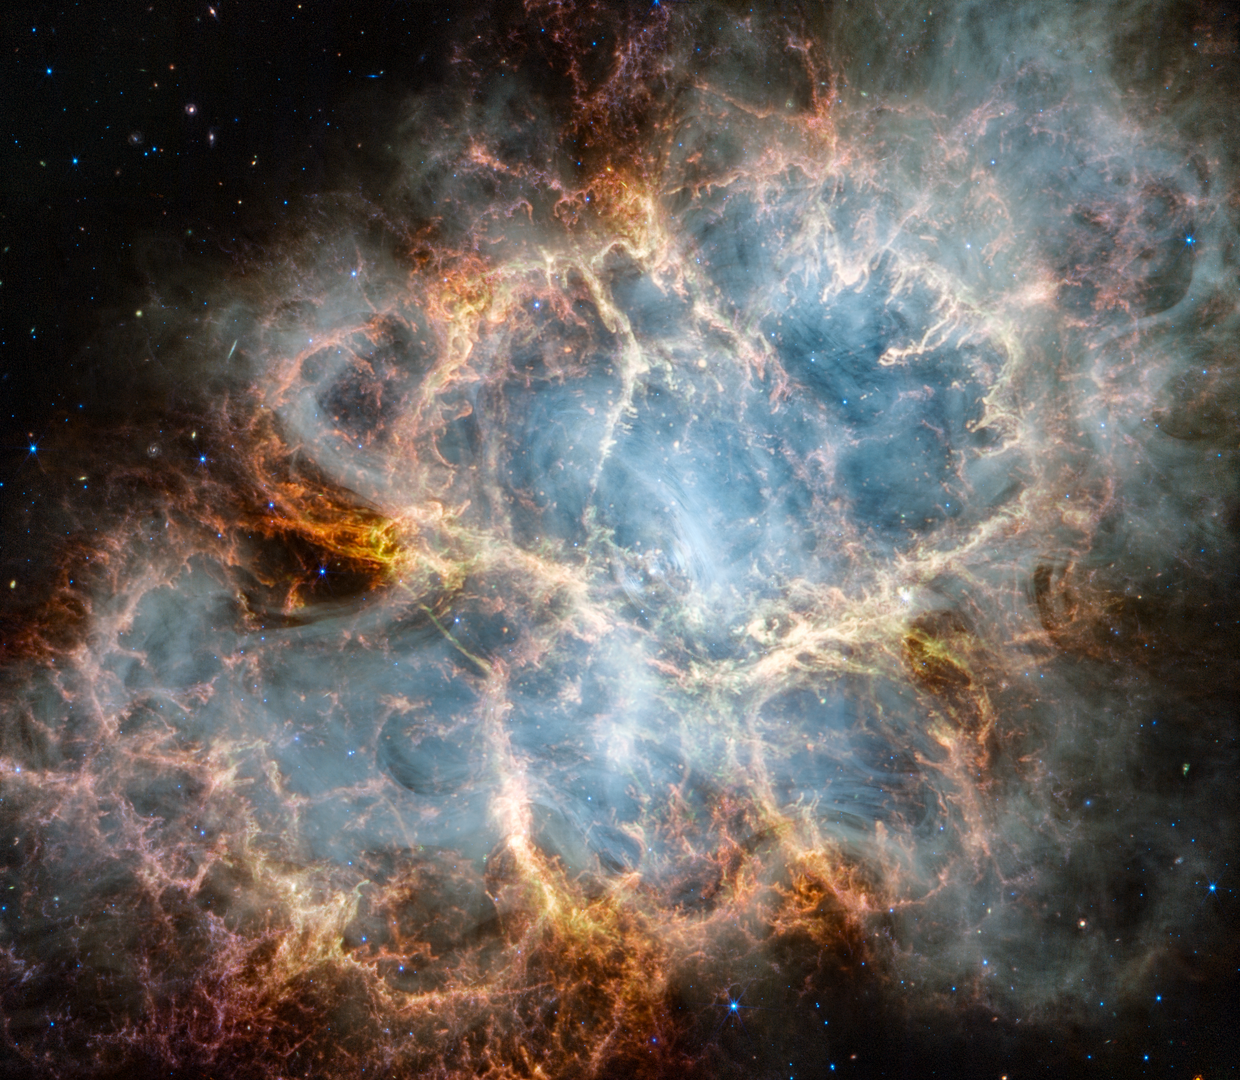
\includegraphics[width=0.5\textwidth]{1240px-Crab_Nebula_imaged_using_James_Webb_Space_Telescope.png}
                \caption{\small{Crab Nebula imaged using James Webb Space Telescope in infrared via its NIRCam (Near-Infrared Camera) and MIRI (Mid-Infrared Instrument).}}
            \end{wrapfigure}

            \phantom{0}\\
            \phantom{0}\\
            \phantom{0}\\
            \phantom{0}\\
            \phantom{0}\\


            \textbf{\noindent The Crab Nebula

            \noindent The first identified source beyond 100 TeV, even PeV.}
            \phantom{0}\\
            \phantom{0}\\
            \phantom{0}\\
            \phantom{0}\\
            \phantom{0}\\
            \phantom{0}\\
            \phantom{0}\\
            \phantom{0}\\
            \phantom{0}\\
            \phantom{0}\\
            \phantom{0}\\
            \phantom{0}\\
            \phantom{0}\\
            \phantom{0}\\
            \phantom{0}\\
            \phantom{0}\\
            \phantom{0}\\
        \end{frame}

    \section{Naima}
        \begin{frame}
            \frametitle{Introduction of Naima}
            \begin{itemize}
                \item \huge{Naima}
            \end{itemize}
            
            \phantom{0}\\

            Naima is a Python package for computation of non-thermal radiation from relativistic particle populations. It includes tools to perform MCMC fitting of radiative models to X-ray, GeV, and TeV spectra using emcee, an affine-invariant ensemble sampler for Markov Chain Monte Carlo. Naima is an Astropy affiliated package.
        \end{frame}

    \section{Some Physics}
        \begin{frame}
            \huge{
            \begin{itemize}
                \item Synchrotron Radiation
                \item Inverse Compton Scattering
                \item Pion Decay
            \end{itemize}}
        \end{frame}

    \section{Results from LHAASO}
        \begin{frame}
            \begin{figure}[t]
                \centering
                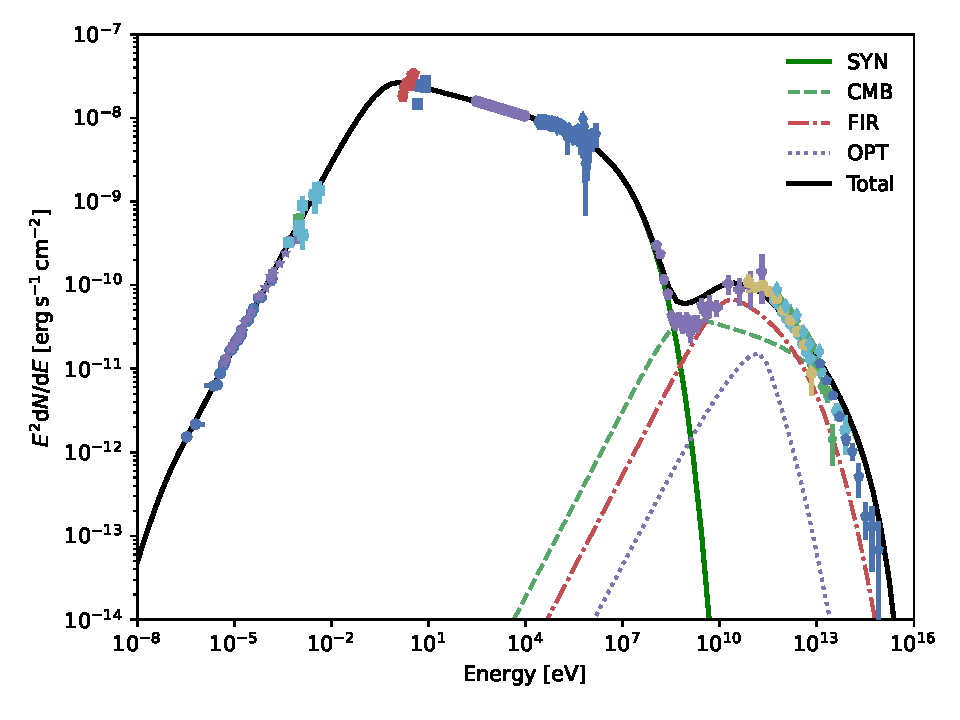
\includegraphics[width=0.8\linewidth]{SynIC-BestFitPar1.pdf}
                \caption{Synchrotron + Inverse Compton distribution of eletrons.}
            \end{figure}
        \end{frame}
        \begin{frame}
            \begin{figure}[t]
                \centering
                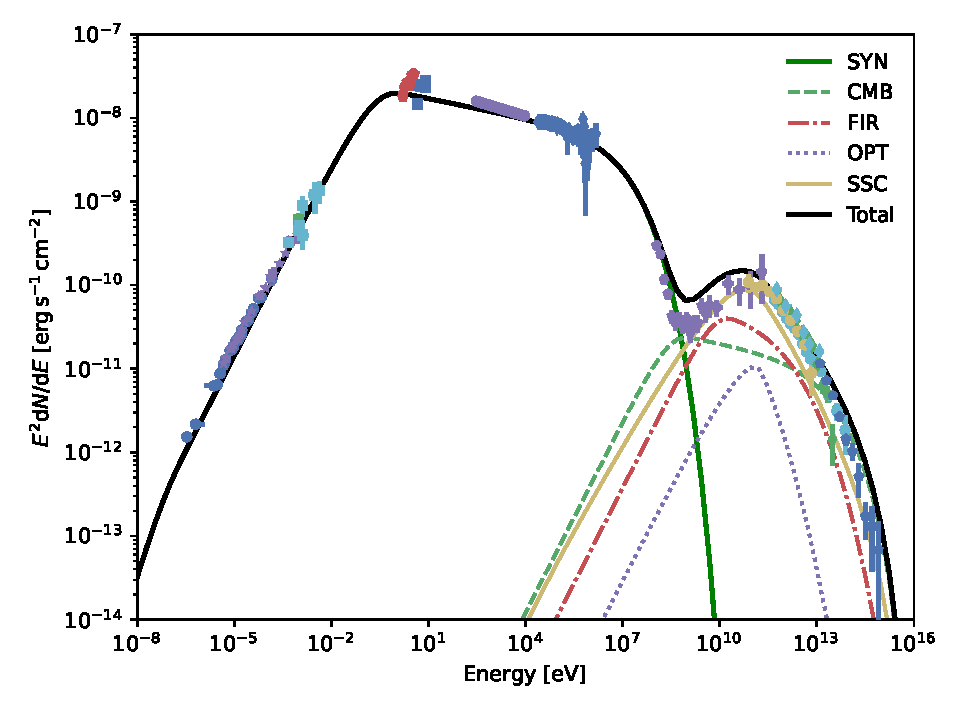
\includegraphics[width=0.8\linewidth]{SynIC-BestFitPar2.pdf}
                \caption{Consider the distribution of Self Synchrotron Compton.}
            \end{figure}
        \end{frame}





    \section{References}
        \begin{frame}
            \begin{thebibliography}{1}
                \bibitem{bib1}
                1
            \end{thebibliography}
        \end{frame}
\end{document}


